% !TEX TS-program = LuaLaTeX+shellescape
% !TEX encoding = UTF-8 Unicode
\RequirePackage{luatex85}
\documentclass[crop=true]{standalone}
\usepackage{pgfplots}
\usepgfplotslibrary{fillbetween}
%\usetikzlibrary{angles}
\pgfplotsset{compat=1.15}
%\pdfminorversion=5 % to allow compression
%\pdfobjcompresslevel=5
%\pdfcompresslevel=14
%\pgfplotsset{
%	layers/my layer set/.define layer set={background,main,foreground}{},set layers=my layer set,}

\begin{document}
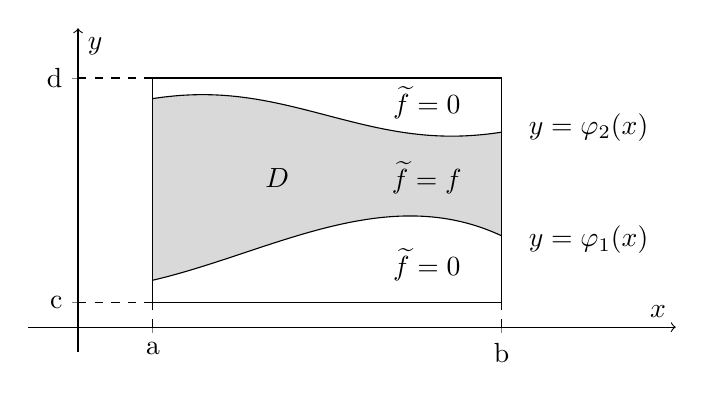
\begin{tikzpicture}[baseline]
\begin{axis}[
axis lines = middle,
unit vector ratio*=2 1 1,
scale=1.2, xmin=-0.2, xmax=2.4, ymin=-0.2, ymax=2.4,
%grid = major,
xtick={0.3,1.7},
ytick={0.2,2},
xticklabels = {a,b},
yticklabels = {c,d},
xlabel=$x$,
ylabel=$y$,
axis line style = {->},
]
\addplot[name path=up,samples=100,domain=0.3:1.7]{1.7+sin(deg(pi*x))/6};
\addplot[name path=below,samples=100,domain=0.3:1.7]{0.3+x^2-1/2*x^3};
%\addplot[name path=xaxis,domain=0:2]{0};
%\draw[thick](axis cs:1,0) -- (axis cs:1,3);
\addplot[gray!30]fill between[of=up and below,soft clip={domain=0.3:1.7}];
%\draw[thick](axis cs:0.2,0.4) rectangle (axis cs:2.4,2.3);
%\coordinate (A) at (axis cs:1,0);
%\coordinate (B) at (axis cs:0,0);
%\coordinate (C) at (axis cs:0.86602540378,0.5);
\draw[] (axis cs:0.3,0.2) -- (axis cs:0.3,2) -- (1.7,2) -- (axis cs:1.7,0.2) -- cycle;
\draw[thin,dashed] (axis cs:0.3,0) -- (axis cs:0.3,0.2);
\draw[thin,dashed] (axis cs:1.7,0) -- (axis cs:1.7,0.2);
\draw[thin,dashed] (axis cs:0,0.2) -- (axis cs:0.3,0.2);
\draw[thin,dashed] (axis cs:0,2) -- (axis cs:0.3,2);
%\pic[draw,angle radius=0.5cm,angle eccentricity=1.5]{angle = A--B--C};
\node at (axis cs:0.8,1.2){$D$};
\node at (axis cs:2.05,0.7){$y=\varphi_1(x)$};
\node at (axis cs:2.05,1.6){$y=\varphi_2(x)$};
\node at (axis cs:1.4,1.2){$\widetilde{f}=f$};
\node at (axis cs:1.4,0.5){$\widetilde{f}=0$};
\node at (axis cs:1.4,1.8){$\widetilde{f}=0$};
\end{axis}
\end{tikzpicture}

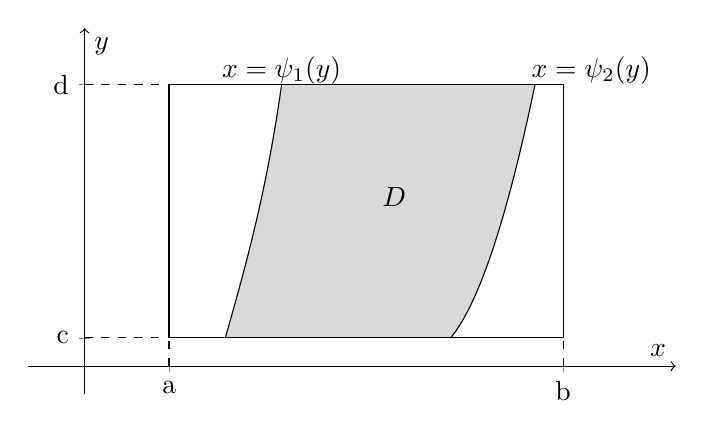
\begin{tikzpicture}[baseline]
\begin{axis}[
axis lines = middle,
unit vector ratio*=2 1 1,
scale=1.2, xmin=-0.2, xmax=2.1, ymin=-0.2, ymax=2.4,
%grid = major,
xtick={0.3,1.7},
ytick={0.2,2},
xticklabels = {a,b},
yticklabels = {c,d},
xlabel=$x$,
ylabel=$y$,
axis line style = {->},
]
\addplot[name path=left,samples=100,domain=0.5:0.7]{0.2+1.8*tan(deg(pi*(x-0.5)*1.25))};
\addplot[name path=right,samples=100,domain=1.3:1.6]{0.2-1.8/15+((x-1.2)*10)^2/15*1.8};
\addplot[name path=up,domain=0.7:1.6]{2};
\addplot[name path=down,domain=0.5:1.3]{0.2};
%\draw[thick](axis cs:1,0) -- (axis cs:1,3);
\addplot[gray!30]fill between[of=left and down,domain=0.5:0.7];
\addplot[gray!30]fill between[of=up and down,soft clip={domain=0.7:1.3}];
\addplot[gray!30]fill between[of=right and up,domain=1.3:1.6];
%\draw[thick](axis cs:0.2,0.4) rectangle (axis cs:2.4,2.3);
%\coordinate (A) at (axis cs:1,0);
%\coordinate (B) at (axis cs:0,0);
%\coordinate (C) at (axis cs:0.86602540378,0.5);
\draw[] (axis cs:0.3,0.2) -- (axis cs:0.3,2) -- (1.7,2) -- (axis cs:1.7,0.2) -- cycle;
\draw[thin,dashed] (axis cs:0.3,0) -- (axis cs:0.3,0.2);
\draw[thin,dashed] (axis cs:1.7,0) -- (axis cs:1.7,0.2);
\draw[thin,dashed] (axis cs:0,0.2) -- (axis cs:0.3,0.2);
\draw[thin,dashed] (axis cs:0,2) -- (axis cs:0.3,2);
%\pic[draw,angle radius=0.5cm,angle eccentricity=1.5]{angle = A--B--C};
\node at (axis cs:1.1,1.2){$D$};
\node at (axis cs:0.7,2.1){$x=\psi_1(y)$};
\node at (axis cs:1.8,2.1){$x=\psi_2(y)$};
%\node at (axis cs:1.4,1.2){$\widetilde{f}=f$};
%\node at (axis cs:1.4,0.5){$\widetilde{f}=0$};
%node at (axis cs:1.4,1.8){$\widetilde{f}=0$};
\end{axis}
\end{tikzpicture}


\end{document}